\documentclass[UTF8,a4paper,10pt]{ctexart}
\usepackage[margin=19mm,top=20mm,bottom=20mm]{geometry}
\usepackage{amsmath,amssymb,booktabs,tabularx,graphicx,xcolor,fancyhdr,enumitem,tikz}
\usetikzlibrary{arrows.meta,positioning}
\usepackage[colorlinks=true,linkcolor=teal,urlcolor=teal]{hyperref}
\definecolor{ink}{HTML}{142B43}\definecolor{accent}{HTML}{168579}\definecolor{teal}{HTML}{168579}
\pagestyle{fancy}\fancyhf{}\fancyhead[L]{\small CF2026 Project 2 · 正式研究报告}\fancyhead[R]{\small 青序量化研究平台}
\fancyfoot[L]{\scriptsize 2026-10-19 · 原文复现 / 差异归因 / 固定规则改进}\fancyfoot[R]{\thepage}
\setlength{\headheight}{15pt}\setlength{\parskip}{5pt}\setlength{\emergencystretch}{2em}\setlength{\parindent}{2em}
\setlist{nosep,leftmargin=1.7em}\ctexset{section={format=\Large\bfseries\color{ink}},subsection={format=\normalsize\bfseries\color{accent}}}
\newcommand{\lead}[1]{\par\noindent{\bfseries\color{accent}#1}\par}
\newcommand{\page}[1]{\newpage\section*{#1}}
\begin{document}
\begin{center}{\small\color{accent}COMPUTATIONAL FINANCE / PROJECT 2}\\[8pt]
{\Huge\bfseries\color{ink}RSRS 择时研究}\\[6pt]
{\Large 原文复现、差异归因与波动率仓位控制}\\[8pt]
2026年10月19日\quad 正式课程报告\quad 截止日期：2026年11月1日
\end{center}

12412408 胡博文；12410819 谢明飞；12410436 王天希

\section*{1\quad 摘要与主要结论}
本项目以光大证券2017年5月1日研报为研究对象，将RSRS斜率、标准分、修正分、右偏分和价格过滤规则接入青序P1平台。我们先复核公式及可交易的信息时点，再分别讨论原样本兼容实验、共同区间对照与发表后检验，最后用固定的15\%年化波动率目标调整仓位。
\lead{核心研究发现：暖机约定会改变早期复现，风险改进须与单纯减仓区分。}
原文第22页允许历史不足时使用已有斜率；准备版采用完整窗口暖机，二者不是同一规则。本次保留严格暖机主协议，并增加部分历史窗口兼容实验。原文没有公开精确交易日、完整费用计提和Wind快照，因此本报告不声称逐笔重建原始账户。
\subsection*{主检验：沪深300，2017-05-02至2026-10-15，买卖各10bp}

\begin{center}\small\begin{tabularx}{\textwidth}{Xrrrr}\toprule
策略 & 累计收益 & CAGR & Sharpe & 最大回撤\\\midrule
原右偏+MA & 14.55\% & 1.50\% & 0.179 & 35.01\%\\
固定75\%仓位 & 12.48\% & 1.30\% & 0.180 & 27.31\%\\
15\%波动目标 & 17.92\% & 1.83\% & 0.227 & 32.85\%\\
买入持有 & 21.41\% & 2.15\% & 0.207 & 45.60\%\\
\bottomrule\end{tabularx}\end{center}
主改进相对原右偏+MA：CAGR变化+0.32个百分点，最大回撤变化-2.16个百分点，Sharpe变化+0.048。固定75\%仓位对照用于判断效果是否只是少承担股票风险。
\lead{主端点存在有限改善，但没有确立收益优势。}15\%目标相对原策略改善了CAGR与回撤；固定75\%仓位的最大回撤仍更低。两组配对年化算术日收益差的95\%区间均跨零，不据此声称风险管理创造稳定alpha。
\subsection*{研究结论的适用范围}
全部历史区间已在研究准备中观察。参数在本轮正式运行前固定，仍不构成未知数据上的盲测；近期区间包含在发表后区间中，不能当作独立重复证据。指数点位是研究代理，未加入ETF跟踪误差、分红、最小交易单位、冲击和真实券商成交。收益不保证未来表现。
\subsection*{交付与软件核验}

RSRS相关自动测试56项通过、0项跳过；6项界面自动测试通过；正式页面策略切换、图表与下载已通过浏览器检查，57交易日回放核账通过。
实际完成198组主实验；其中162组与独立账户对齐。另有16组口径诊断、24组源兼容实验与12组波动目标/费用稳健性检查，均保留结果。
报告、16页Beamer、可编辑演示、逐页讲稿、配置、源码、数据说明与聚合证据一同交付。
\page{2\quad 研究问题、来源与课程要求}
\lead{我们复现的是研报中RSRS价格优化策略的核心结论。}
原文：刘均伟、周萧潇，《基于阻力支撑相对强度（RSRS）的市场择时——技术择时系列报告之一》，光大证券，2017-05-01。目标为第19页图25、表5及第20页图26。图25比较三类标准分的价格优化策略；表5汇总收益、风险和交易统计；图26比较成本情景。
\subsection*{三个可回答的问题}
\begin{enumerate}\item 在明确的数据与成交规则下，核心公式、买卖状态及账户结果能否逐层重建？\item 与原文不同的结果，有多少可由暖机、标准化、均线索引、成交时点与费用解释？\item 保留原信号的15\%波动目标，能否改善回撤，代价是什么，是否优于固定减仓？\end{enumerate}

\begin{center}\small\begin{tabularx}{\textwidth}{lX}\toprule
课件要求 & 本项目的对应证据\\\midrule
接入P1（第4页） & cfquant.rsrs接入已有引擎、绩效与reconcile；界面和CLI共用核心。\\
逐层核验（第4页） & 手算OLS与标准分、阈值状态、未来扰动不影响过去、独立账本重建。\\
并排对照（第5页） & 原图25/表5/图26截图与本次同主题输出并排；三层区间分开。\\
差异归因（第6页） & 固定基准、单因素矩阵和实际差值；不能解释的差异明确保留。\\
自主改进（第7页） & 仅改仓位，增加固定75\%仓位对照、费用和波动目标敏感性。\\
可复现提交（第8页） & 原文位置、数据哈希、代码版本、协议、seed、检查结果与材料。\\
\bottomrule\end{tabularx}\end{center}
\subsection*{来源优先级与复用}
研报排版正文是方法依据，第三方手写批注不作为作者陈述。开源QuantsPlaybook用来定位合法公开研究材料与实现差异，不直接运行或复用其账户逻辑。课程要求与原文方法分开审计，文档中写明每个补充假设。
\subsection*{原文内部存在的不一致}
摘要写2005年3月至2017年3月，正文部分段落写至2017年4月，图25横轴从2005-02-18起。摘要1971.05\%、正文1826.13\%与第20页无成本净值19.71也不能机械换算成同一个终值。我们不择取最方便的数字作为唯一原值。

\page{3\quad 指标、状态机与可审计补充假设}
\subsection*{带截距滚动OLS}
对收盘日$t$及此前$N-1$日的高低价拟合
\[H_i=\alpha_t+\beta_tL_i+\varepsilon_i,\quad
\beta_t=\frac{\sum_i(L_i-\bar L)(H_i-\bar H)}{\sum_i(L_i-\bar L)^2},\quad
R_t^2=\frac{[\sum_i(L_i-\bar L)(H_i-\bar H)]^2}{\sum_i(L_i-\bar L)^2\sum_i(H_i-\bar H)^2}.\]
退化窗口保留缺失，不用未来或零值补齐。主规则以严格早于$t$的$M$个有效斜率计算
\[z_t=\frac{\beta_t-\mu_{t-1,M}}{\sigma_{t-1,M}},\qquad
z_t^{\mathrm{corr}}=z_tR_t^2,\qquad z_t^{\mathrm{right}}=z_tR_t^2\beta_t.\]
主标准差为总体口径ddof=0；原文明确早期可使用部分历史，但未明确是否含当日、ddof和最低有效样本数，故单独做控制实验。

\begin{center}\small\begin{tabularx}{\textwidth}{Xlll}\toprule
信号 & N / M & 入场 / 出场 & 价格过滤\\\midrule
原始斜率 & 18 / 无 & \ensuremath{\beta} > 1.0 / \ensuremath{\beta} < 0.8 & 无\\
标准分、修正分 & 18 / 600 & >0.7 / <\ensuremath{-}0.7 & 另列MA版本\\
右偏分 & 16 / 300 & >0.7 / <\ensuremath{-}0.7 & 主候选增加MA\\
MA入场条件 & 20日均线 & MA[t] > MA[t\ensuremath{-}2] & 不因MA下降强制卖出\\
\bottomrule\end{tabularx}\end{center}
\subsection*{持仓状态与执行}
空仓时只有信号超过上阈值且入场条件成立才开仓；持仓时信号低于下阈值才退出，其余时间延续状态。主候选right\_ma不是“每天挑最高分股票”，而是单一指数做多/现金的滞回状态机。
收盘$t$计算信号，$t+1$开盘成交，$t+1$收盘估值。单边成本按实际成交金额收取，现金利息和无风险收益率均为0，无杠杆，不强制末日清仓。次日开盘和费用是本项目补充约定，不是研报已完全规定的细节。
\subsection*{价格过滤的索引歧义}
原文同时使用“前一日/前三日”与“当日/3日前”的文字。主规则按执行日解释为MA[t]与MA[t−2]；lag=3只作独立敏感性。原文均线过滤已有，不列为本组创新。

\page{4\quad 数据快照与三层比较范围}
\lead{先确定什么可以比较，再解释收益差异。}
本次复用研究准备版的三个指数公开日频快照：沪深300、上证50、中证500，来源为Tencent Finance公共行情。该指数研究与P1个股Tushare快照分开；不会把供应商更换本身写成已识别的收益原因。

\begin{center}\scriptsize\begin{tabularx}{\textwidth}{Xrlll}\toprule
指数 & 记录数 & 首日 & 末日 & 缺失/重复\\\midrule
沪深300 & 5288 & 2005-01-04 & 2026-10-15 & 0/0\\
上证50 & 5531 & 2004-01-02 & 2026-10-15 & 0/0\\
中证500 & 5288 & 2005-01-04 & 2026-10-15 & 0/0\\
\bottomrule\end{tabularx}\end{center}
\begin{center}\small\begin{tabularx}{\textwidth}{lXX}\toprule
层次 & 区间与规则 & 能回答的问题\\\midrule
原样本兼容 & 2005-03-01至2017-03-31；另测4月末 & 部分历史暖机，贴近原图/表；首尾和Wind仍不完全同源。\\
共同区间 & 2007-08-01至2017-03-31；严格暖机 & 同一输入、费用和账户下比较各信号及控制。\\
发表后检验 & 2017-05-02至2026-10-15；严格暖机 & 方法发布后是否保持效果；本次已观察的历史。\\
近期敏感性 & 2020-01-02至2026-10-15 & 市场阶段影响；与上一层重叠，不能视作独立样本。\\
\bottomrule\end{tabularx}\end{center}
\subsection*{部分历史窗口兼容实验}
原文第22页明确举例：标准化历史不足600日时，用已有的斜率。兼容实现仍需至少两个有效斜率及非零标准差，沿用排除当日、ddof=0；这只还原已知的早期窗口原则，不能消除全部未公开细节。严格暖机与部分暖机的区别在同一期间、同一费用下单独比较。
\subsection*{数据质量与身份}
日期要求升序、唯一、无时区且对应日频记录；OHLC必须有限且为正，最高价不得低于最低价。不填补缺失交易日，不以最新值倒填历史。快照SHA-256、行数、日期范围和研究文件哈希随证据包保存，重跑先验证输入身份。
\subsection*{价格指数的经济含义}
研究按连续指数单位交易，输入无个股涨跌停或容量约束，价格指数没有直接持有工具和分红再投资。该账本可检验信号及资金会计，但不能称作可立即执行的ETF策略或沪深300全收益投资。可交易扩展应另加ETF实际OHLC、费率、分红和跟踪误差。
\subsection*{结论的独立性}
正式协议固定主端点、15\%目标、20日窗口、75\%降仓对照、有限敏感性及重采样seed；准备版已观察同段历史，因此“先写协议”提高本轮透明度，并不把既有历史转换成盲测。

\page{5\quad 公式手算、因果性与账户核验}
\lead{净值曲线之前，先验证每一个会影响交易的中间量。}
\subsection*{可手算的OLS例子}
取$L=(1,2,3)$，$H=(2,3,5)$，则$\bar L=2$、$\bar H=10/3$，
\[\sum(L-\bar L)^2=2,\quad\sum(L-\bar L)(H-\bar H)=3,\quad
\sum(H-\bar H)^2=14/3.\]
因而$\beta=3/2$，$\alpha=1/3$，$R^2=27/28\approx0.964286$。如果此前斜率为$(1,2,3)$，当前$\beta=4$，则$z=(4-2)/\sqrt{2/3}=\sqrt6$。这些小例子只验证公式，不代表可投资样本。

\subsection*{真实窗口的独立复算}形成日2017-04-28，执行日2017-05-02；独立最小二乘重复计算16日窗口和此前300个斜率。$\beta=0.833201$，$R^2=0.891854$，$z=-0.160262$，右偏分$-0.119090$；最大绝对误差为7.88e-15，小于预定$10^{-8}$容差。16个观测点、残差和此前斜率日期均可核对。

\subsection*{核验层次}

\begin{center}\small\begin{tabularx}{\textwidth}{lX}\toprule
层次 & 检查方法与通过含义\\\midrule
公式 & 向量化OLS对照逐窗独立计算；beta、R\textsuperscript{2}、z及变换均保存。\\
信号 & 阈值上下穿越、缺失窗口、MA仅限制入场；手工状态序列可对照。\\
因果 & 扰动未来价格不应改变此前指标、目标和交易；信号日严格早于成交日。\\
账户 & 逐笔成交重建份额、现金、费用和净值；无负现金或超过100\%目标。\\
独立参照 & P1共享账本与准备版独立账户同输入比较；差异不得直接跳过。\\
产物 & 结果、协议、输入身份与配置一同留存；软件测试与研究表现分开。\\
\bottomrule\end{tabularx}\end{center}
\subsection*{绩效口径}
设每日净值$V_t$、初始资金$V_0$、交易日数$T$，日收益$r_t=V_t/V_{t-1}-1$，则
\[\mathrm{CAGR}=(V_T/V_0)^{252/T}-1,\quad
\mathrm{Sharpe}=\sqrt{252}\,\bar r/s(r),\quad
\mathrm{MDD}=\max_t\left(1-\frac{V_t}{\max_{u\le t}V_u}\right).\]
Sharpe使用日收益样本标准差（ddof=1）、无风险利率0；最大回撤报告为正的损失幅度，原表用负号。初始资金纳入回撤峰值。换手按成交名义金额除以账户规模，不能把成交笔数等同于完整往返次数。

\page{6\quad 图25：原文与本次兼容实验并排}
\lead{原文展示高净值；本次输出必须连同样本与假设一起阅读。}

\begin{center}\begin{minipage}[t]{.49\textwidth}\centering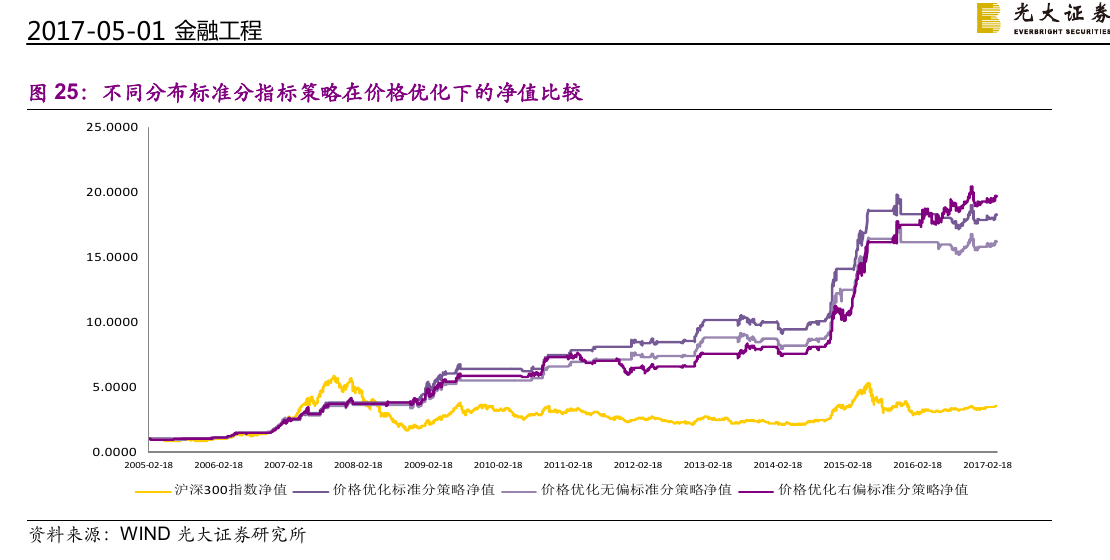
\includegraphics[width=\linewidth,height=73mm,keepaspectratio]{figures/source_figure25.png}\end{minipage}\hfill\begin{minipage}[t]{.49\textwidth}\centering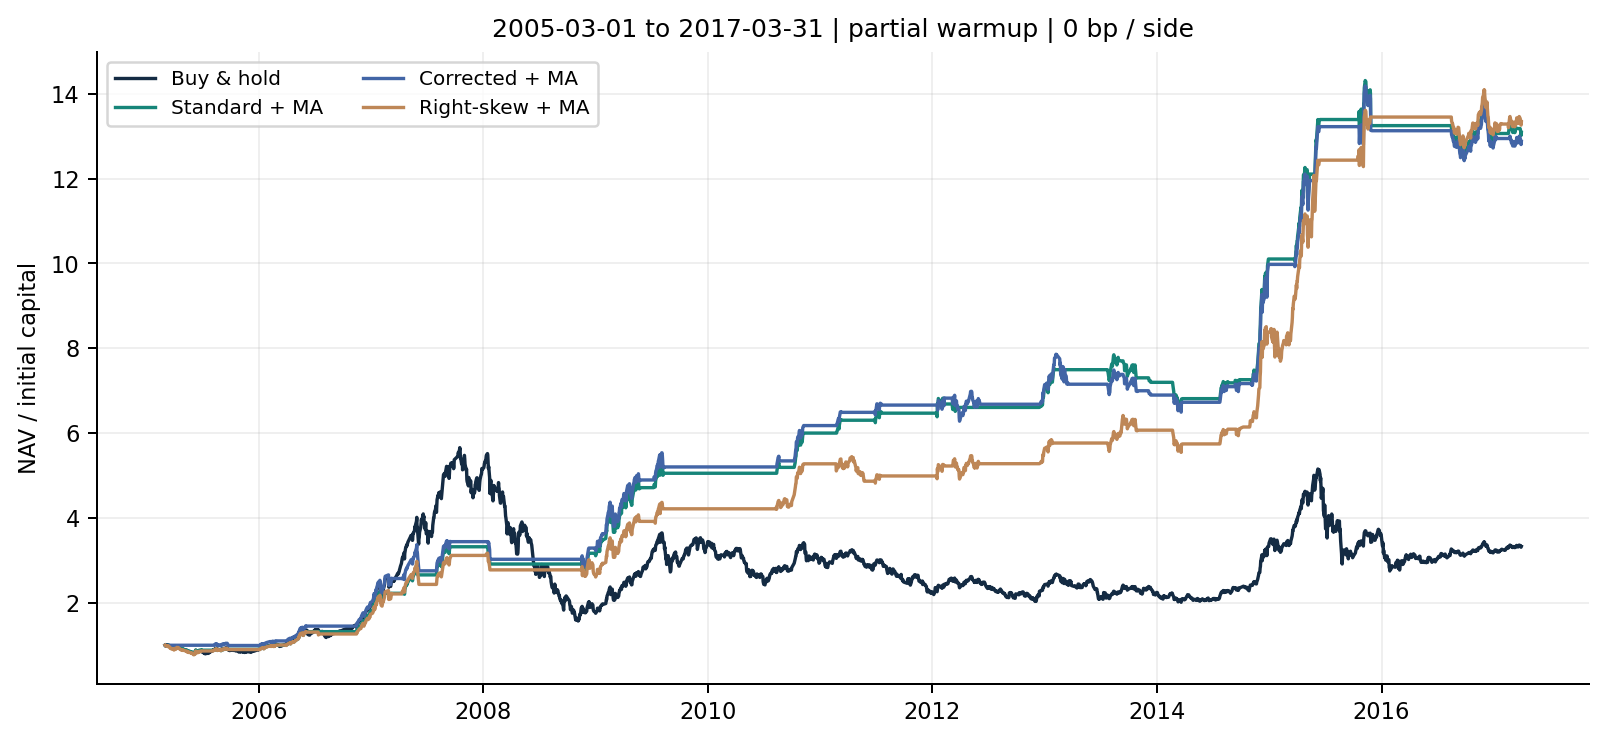
\includegraphics[width=\linewidth,height=73mm,keepaspectratio]{figures/reproduction_curves.png}\end{minipage}\end{center}
\noindent\small 左：原文第19页图25截图，保留标题、图例和WIND/光大证券研究所来源行。右：2005-03-01至2017-03-31，本次指数快照、部分历史暖机、零成本、次日开盘；相同主题不代表完全相同口径。\normalsize
\begin{center}\small\begin{tabularx}{\textwidth}{Xrrrr}\toprule
候选（兼容区间） & 累计收益 & CAGR & Sharpe & 最大回撤\\\midrule
标准分+MA & 1208.73\% & 24.65\% & 1.560 & 20.79\%\\
修正分+MA & 1187.30\% & 24.48\% & 1.505 & 18.26\%\\
原右偏+MA & 1233.27\% & 24.85\% & 1.404 & 22.96\%\\
\bottomrule\end{tabularx}\end{center}
\subsection*{可检验的复现内容}
三类标准分、MA入场过滤与相同阈值都落实到代码中，指标和交易状态可下载逐日检查。右偏版本同时改变N/M，所以与标准分的差异不是单独乘beta的纯效应；这个限制在比较表中明确保留。
\subsection*{无法消除的可比性差异}
Wind原始行情、确切首末日、当日是否参与标准化及完整成交模型未公开。我们没有原始逐日净值去验证逐点误差。图形形状相似或累计收益接近都不是“完全复现”的充分条件；不同费用、暖机和交易时点的控制实验见后文。

\page{7\quad 表5：原始统计与本次统计的边界}
\begin{center}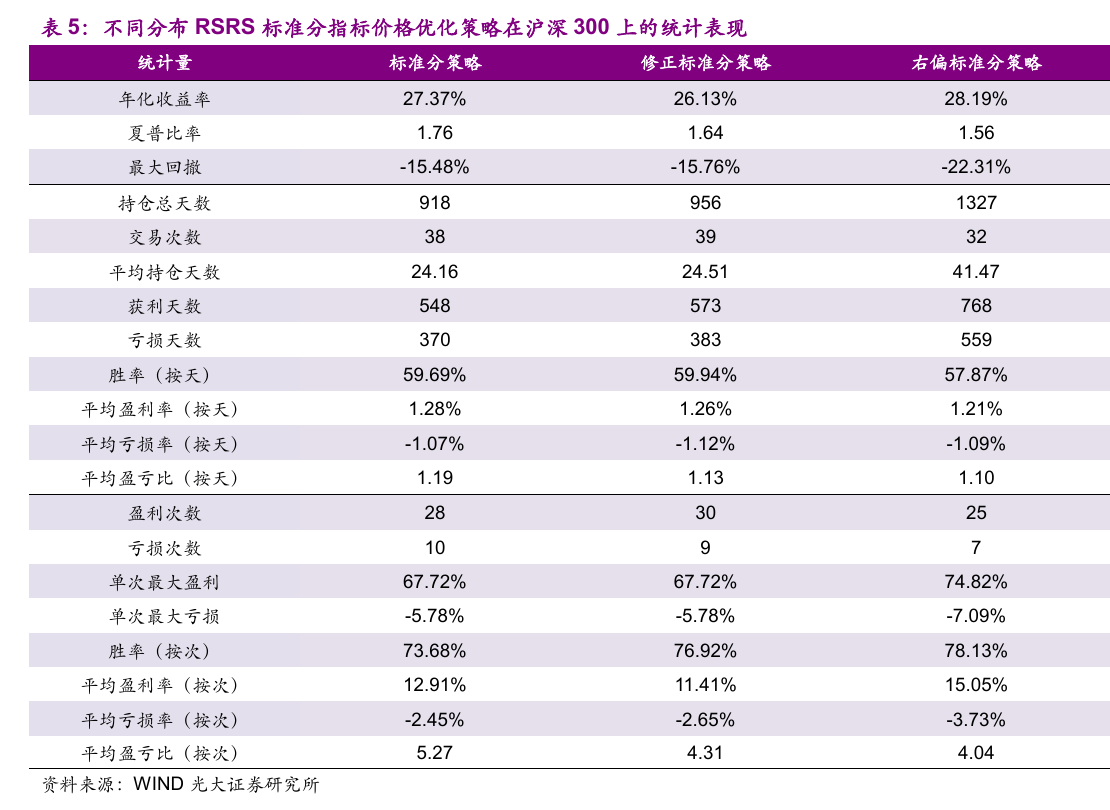
\includegraphics[width=.83\textwidth,height=110mm,keepaspectratio]{figures/source_table5.png}\end{center}
\noindent\small 上：原文第19页表5完整截图，保留20个统计量及来源。全文抄录固定在来源审计，不用当前结果覆盖原表。\normalsize
\subsection*{同定义可解释的比较}
主要对照CAGR、Sharpe、最大回撤；回撤统一为正损失幅度。交易次数需区分成交笔数、入场次数和已结束往返，原文“持仓日”与开盘/收盘有仓日也可能不同。本次列取自reproduction\_table.csv，不把尚未对齐口径的两列差值称作估计误差。

\begin{center}\scriptsize\begin{tabularx}{\textwidth}{Xrrrrrr}\toprule
价格优化候选 & 原年化 & 本次年化 & 原Sharpe & 本次Sharpe & 原回撤 & 本次回撤\\\midrule
标准分+MA & 27.37\% & 24.65\% & 1.76 & 1.560 & 15.48\% & 20.79\%\\
修正分+MA & 26.13\% & 24.48\% & 1.64 & 1.505 & 15.76\% & 18.26\%\\
原右偏+MA & 28.19\% & 24.85\% & 1.56 & 1.404 & 22.31\% & 22.96\%\\
\bottomrule\end{tabularx}\end{center}
\small 本次列：2005-03-01至2017-03-31、部分历史窗口、零成本、次日开盘，与reproduction\_table.csv一致。2017-04-28截止仅列为端点敏感性。原文列的精确样本、费用和标准差细节未完全公开。\normalsize
\page{8\quad 图26：费用敏感性与可交易假设}

\begin{center}\begin{minipage}[t]{.49\textwidth}\centering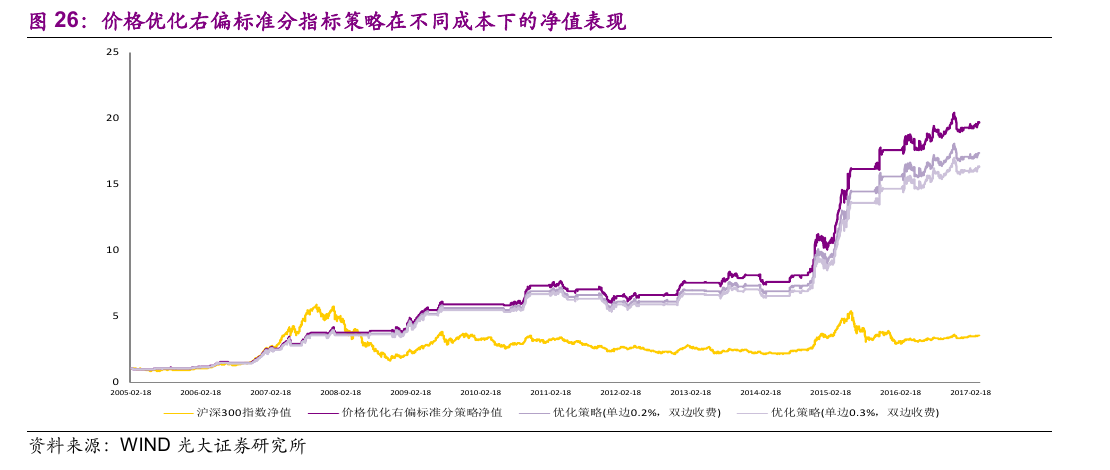
\includegraphics[width=\linewidth,height=78mm,keepaspectratio]{figures/source_figure26.png}\end{minipage}\hfill\begin{minipage}[t]{.49\textwidth}\centering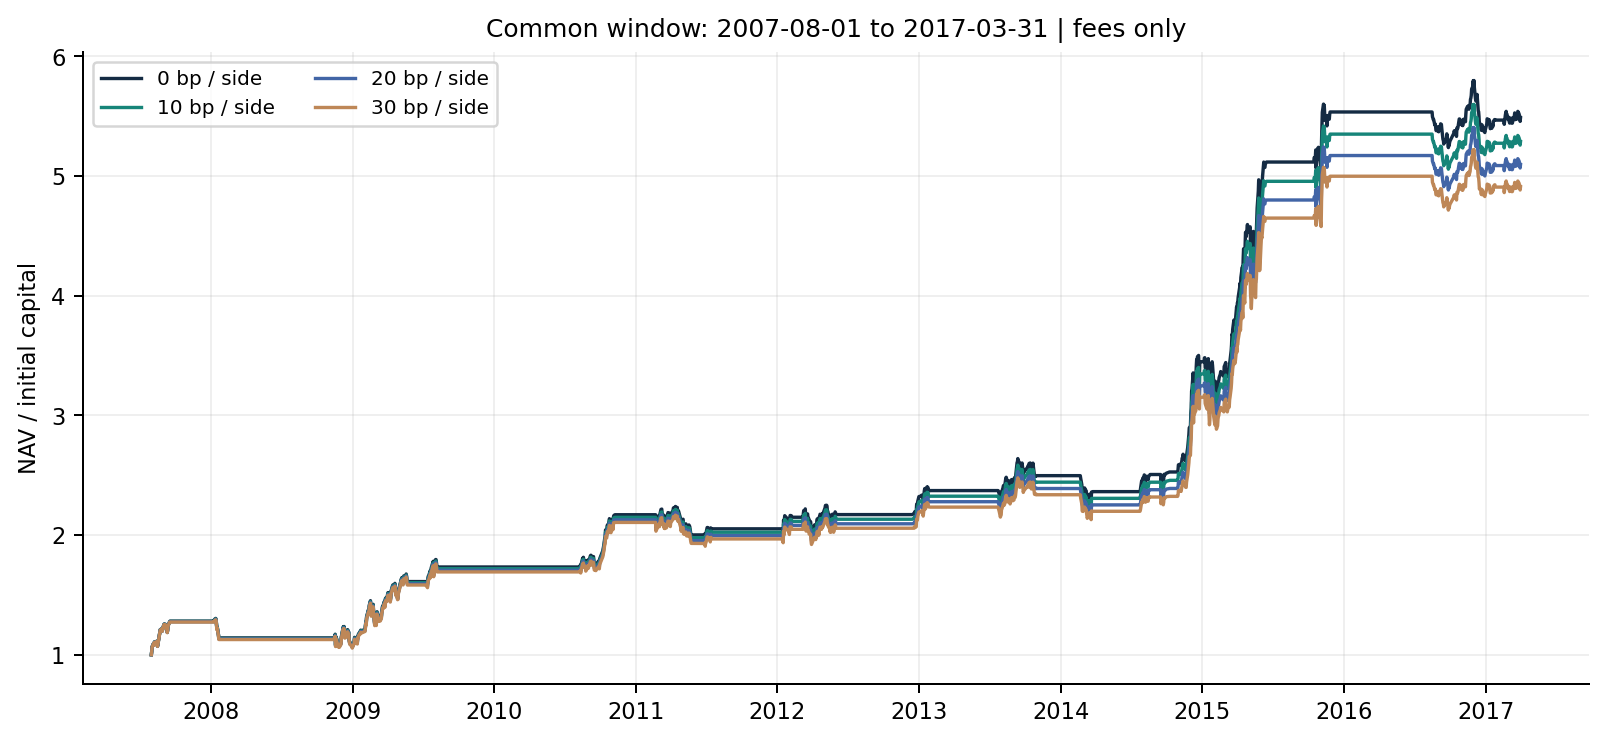
\includegraphics[width=\linewidth,height=78mm,keepaspectratio]{figures/cost_curves.png}\end{minipage}\end{center}
\small 左：原文第20页图26，原图例为零成本及单边0.2\%/0.3\%双边收取。右：本次共同区间2007-08-01至2017-03-31，0/10/20/30bp每边。样本不同，费用水平可映射；原文具体计提仍不完全公开。\normalsize
\begin{center}\small\begin{tabularx}{\textwidth}{Xrrrr}\toprule
每边成本 & 累计收益 & CAGR & Sharpe & 最大回撤\\\midrule
0 bp & 448.69\% & 20.01\% & 1.280 & 17.79\%\\
10 bp & 428.76\% & 19.53\% & 1.254 & 17.95\%\\
20 bp & 409.55\% & 19.06\% & 1.227 & 18.12\%\\
30 bp & 391.04\% & 18.59\% & 1.201 & 18.28\%\\
\bottomrule\end{tabularx}\end{center}
\subsection*{怎样解释这张图}
每次只改变费率，信号、样本和执行时点保持一致。费用不仅直接减少现金，也改变此后可买份额，因此长期差值不能简单用“交易次数乘固定金额”复原。更高费率的结果不是另一套经过择优的策略。
\subsection*{次日开盘与次日收盘}
主结果只使用收盘形成、下一开盘成交。控制实验保持信号在$t$收盘形成，把成交推迟至$t+1$收盘，重新计算持仓、费用及买持基准。该对照仍有完整一日滞后，不使用同日收盘抢先交易。指数没有可直接交易账户，实际ETF扩展需独立验证。

\page{9\quad 差异归因：有限单因素实验}
\lead{先排除公式错误，再量化口径差异；对照之间存在相互作用。}
全部对照以固定基准为参照，保留不改善和零差异结果。暖机在原样本兼容阶段尤为关键；共同区间已拥有充足历史时，严格与部分窗口可能趋同，不据此否认早期影响。

\begin{center}\scriptsize\begin{tabularx}{\textwidth}{Xrrr}\toprule
唯一改变 & \ensuremath{\Delta}CAGR(pp) & \ensuremath{\Delta}Sharpe & \ensuremath{\Delta}MDD(pp)\\\midrule
共同区间基准 & +0.00 & +0.000 & +0.00\\
标准化纳入当日 & +0.00 & +0.000 & +0.00\\
样本标准差ddof=1 & +0.00 & +0.000 & +0.00\\
MA比较滞后3日 & -0.30 & -0.009 & +0.00\\
次日收盘成交 & -0.58 & -0.046 & +6.33\\
零成本 & +0.47 & +0.026 & -0.16\\
20bp/边 & -0.47 & -0.027 & +0.16\\
30bp/边 & -0.94 & -0.053 & +0.33\\
\bottomrule\end{tabularx}\end{center}
\subsection*{原样本区间的暖机对照：零成本，截止2017-03-31}
\begin{center}\scriptsize\begin{tabularx}{\textwidth}{Xrrrr}\toprule
候选 & 严格CAGR & 部分CAGR & \ensuremath{\Delta}CAGR(pp) & \ensuremath{\Delta}MDD(pp)\\\midrule
标准分+MA & 14.65\% & 24.65\% & +10.00 & +3.30\\
修正分+MA & 14.14\% & 24.48\% & +10.34 & +0.88\\
原右偏+MA & 23.97\% & 24.85\% & +0.88 & +4.70\\
\bottomrule\end{tabularx}\end{center}
\subsection*{哪些差异能够归因}
在相同数据下，改变标准化是否含当日、ddof、MA lag、费用或成交时点得到的差值，是该设定在指定样本和其他设定固定条件下的影响。它不证明原文采用其中某个未披露口径，也不能外推为所有市场阶段的固定效应。
\subsection*{哪些差异仍未解释}
由于未取得Wind原始快照，不能把剩余差距统称为数据供应商效应；也没有原作者代码证明其早期窗口最低样本数、波动率分母或日收益记账方式。对照作用有相互影响，禁止把各差值直接相加解释原文全部差距。
\subsection*{为何保留较差结果}
课程要求检验和解释，而非只展示收益最高曲线。固定主信号后，其余标准分、均线、暖机、费率和波动目标均保留在完整结果中，避免在看过最终区间后改写主候选或只报告冠军。

\page{10\quad 自主改进：保留信号，调整风险仓位}
\lead{创新点是仓位映射；MA入场过滤来自原文。}
令原右偏+MA二值信号为$s_t\in\{0,1\}$，以截至$t$的20个日收益样本标准差估计年化波动率：
\[\widehat\sigma_t=\sqrt{252}\,s(r_{t-19:t}),\qquad
w_t=s_t\min\{1,0.15/\widehat\sigma_t\}.\]
信号与波动率均在收盘可得，次日开盘将账户调整至目标，允许现金、不加杠杆。缺少完整20日收益时目标为0；完整窗口若波动为0则比例上限为1，不除以零。每日调整可能增加换手。

\begin{center}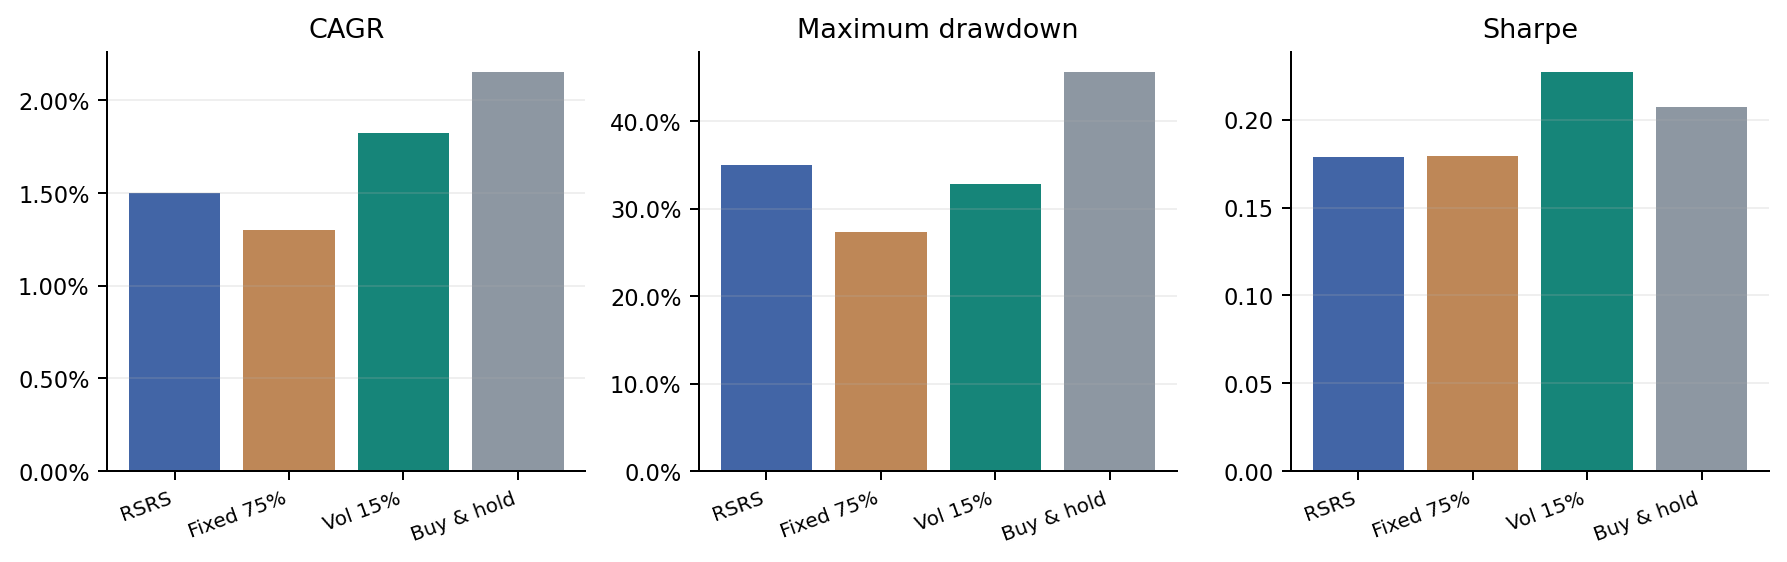
\includegraphics[width=.96\textwidth,height=57mm,keepaspectratio]{figures/main_metrics.png}\end{center}
\begin{center}\small\begin{tabularx}{\textwidth}{Xrrrr}\toprule
发表后主端点 & 累计收益 & CAGR & Sharpe & 最大回撤\\\midrule
原右偏+MA & 14.55\% & 1.50\% & 0.179 & 35.01\%\\
固定75\%仓位 & 12.48\% & 1.30\% & 0.180 & 27.31\%\\
15\%波动目标 & 17.92\% & 1.83\% & 0.227 & 32.85\%\\
买入持有 & 21.41\% & 2.15\% & 0.207 & 45.60\%\\
\bottomrule\end{tabularx}\end{center}
波动目标相对原策略的回撤变化-2.16个百分点，CAGR变化+0.32个百分点。相对固定75\%仓位，回撤变化+5.54个百分点，CAGR变化+0.53个百分点；固定75\%的回撤更低。
原策略、固定75\%与波动目标的年化换手分别为4.61、3.65、5.46倍；平均形成目标分别为48.26\%、36.19\%、42.33\%。
\subsection*{控制实验解释}
固定75\%仓位使用相同二值信号并每日调仓，控制纯粹降低市场暴露的效果；其余25\%现金不计息。它仍未与波动目标精确匹配平均暴露或逐日换手，因此不能独立证明主动波动管理产生alpha。主评价是回撤，收益、Sharpe和换手必须同时报告。

\page{11\quad 发表后净值与跨指数检查}

\begin{center}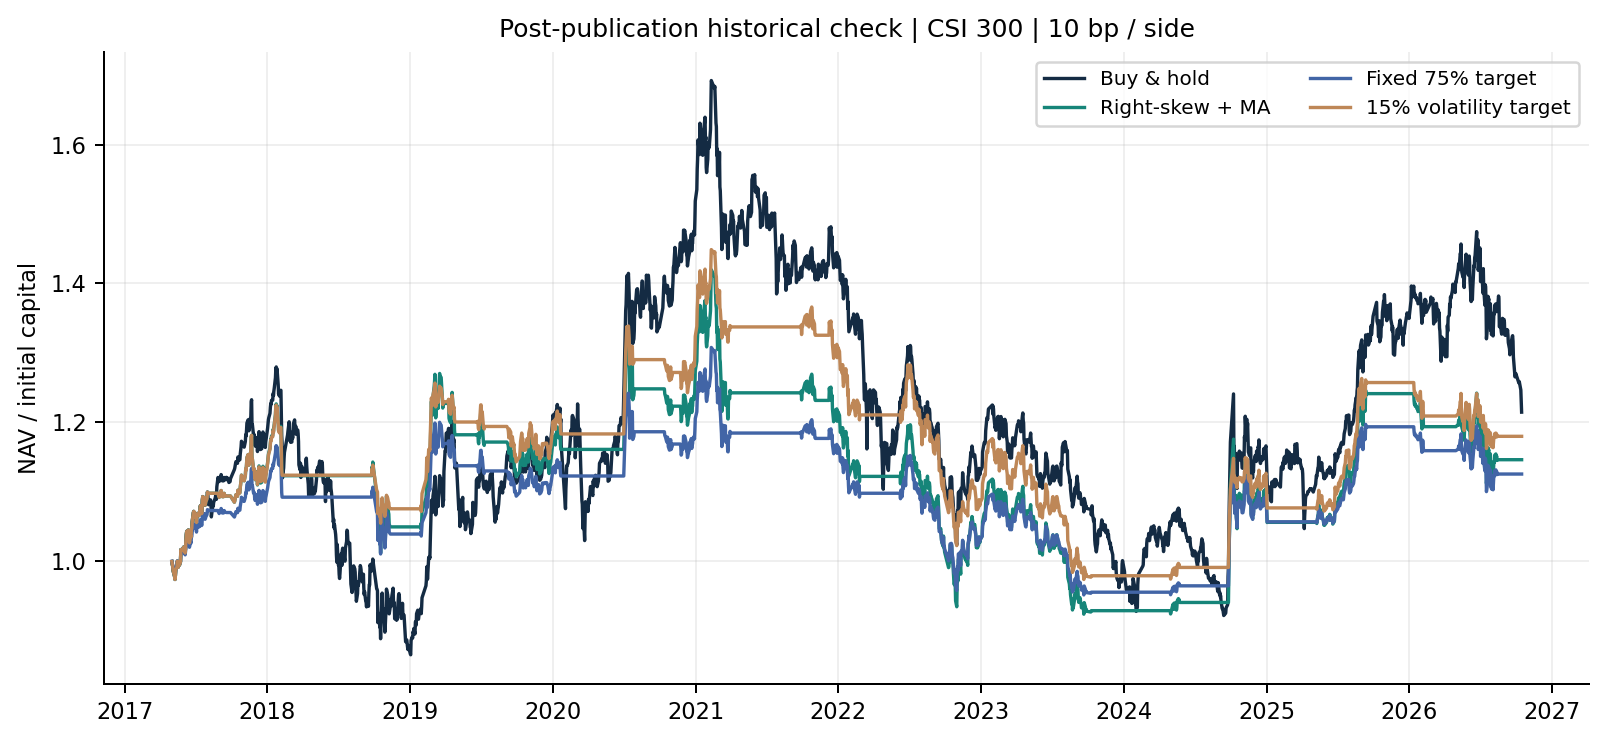
\includegraphics[width=.96\textwidth,height=73mm,keepaspectratio]{figures/main_curves.png}\end{center}
\small 沪深300，2017-05-02至2026-10-15，买卖各10bp；初始资金相同，现金不计息。固定75\%与波动目标均每日调整；原RSRS只在状态改变时交易。\normalsize
\begin{center}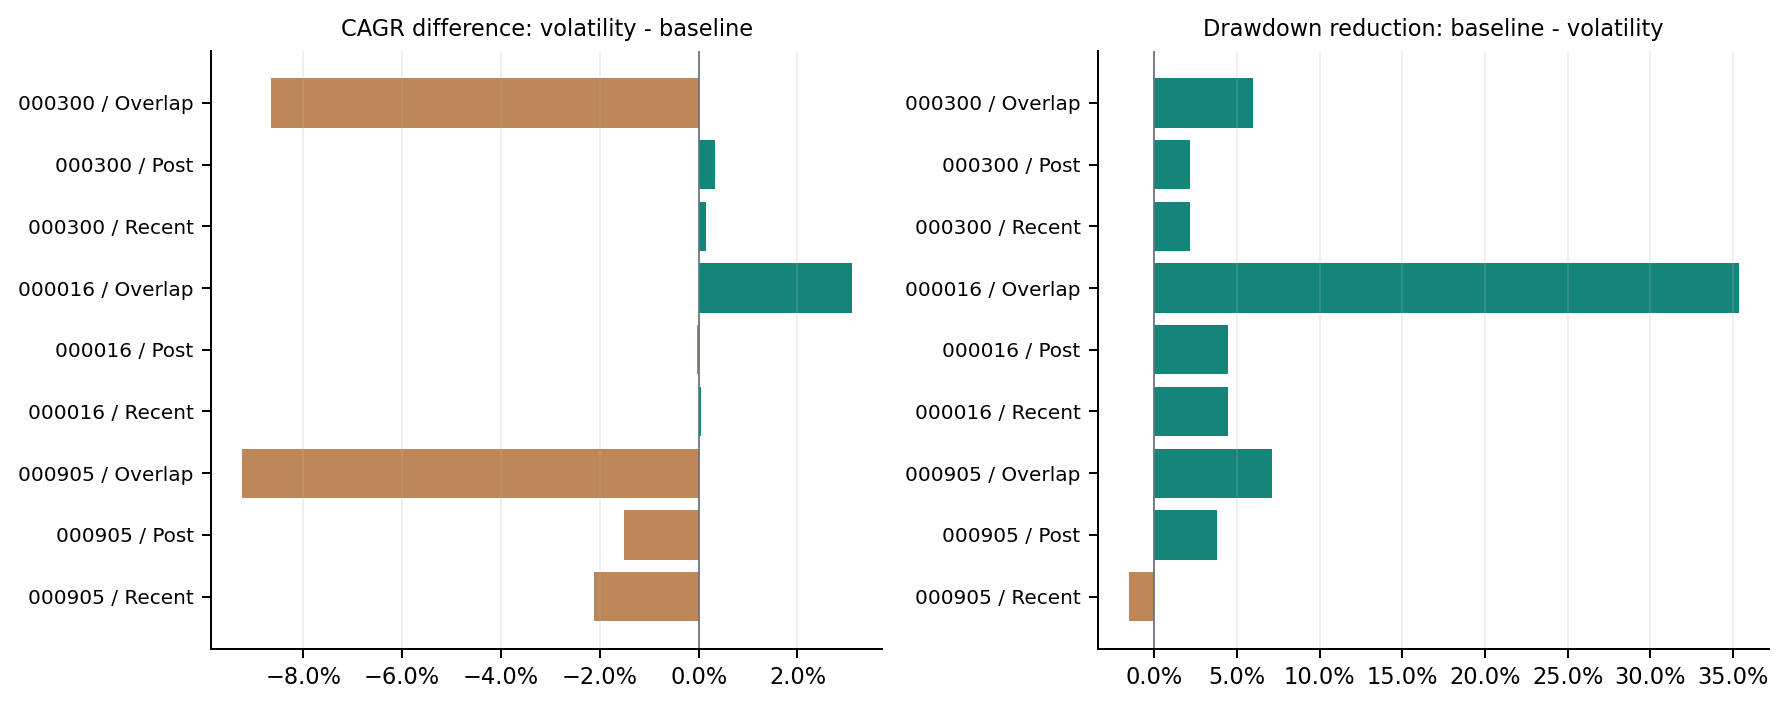
\includegraphics[width=.96\textwidth,height=72mm,keepaspectratio]{figures/robustness.png}\end{center}
\small 上图每组对照共享数据、样本和10bp成本。CAGR差值=波动目标−基准，回撤改善=基准MDD−波动目标MDD，二者分别判断。共同区间、发表后与近期历史互有联系，三指数也高度相关，不能把九组结果当九次独立实验。\normalsize
\subsection*{稳健性而非重新选优}
10\%和20\%目标只检查15\%附近敏感性，不在此后挑最高收益目标替换主方案；零成本与双倍费率检验成本依赖。完整矩阵在performance.csv和paired\_comparison.csv中保留，本文突出研究问题而非隐藏失败案例。

\page{12\quad 不确定性、重采样与失败保留}
\lead{历史差值不是已确立的未来优势。}
使用配对区块重采样：将基准与改进的同日收益一起抽取，保留两策略同期关联；区块长度20个交易日，1000次，随机seed为20261019。百分位区间只描述这一历史收益序列的重采样不确定性，不替代新的前向样本。

\noindent 指标为252倍配对日收益差的算术均值，单位为百分点，\textbf{不是CAGR差值}。\begin{center}\small\begin{tabularx}{\textwidth}{Xrr}\toprule
比较 & 年化算术均值差(pp) & 95\%区间(pp)\\\midrule
15\%目标 \ensuremath{-} 原右偏+MA & -0.02 & [-1.80, +1.72]\\
15\%目标 \ensuremath{-} 固定75\%仓位 & +0.56 & [-1.02, +2.20]\\
\bottomrule\end{tabularx}\end{center}
\subsection*{重采样的局限}
市场结构变化、择时信号的长记忆、策略开发与多重比较均未被短区块完全建模。重采样后的收益路径不是重新按OHLC计算信号并成交的完整新市场，因此仅作描述性配对评价。区间跨零时尤其不能称为稳健改进；不跨零也不能证明可交易未来收益。
\subsection*{保留的负面证据}
主改进如果降低回撤但削弱收益，应陈述风险与收益交换；如果固定75\%已达到相近或更好效果，应把简单降仓列为有力替代。原研报的高年化数字与发表后较弱表现可以同时存在，不能用新时段表现否定公式实现，也不能用原文高收益忽略后续退化。
\subsection*{未进行的再优化}
没有依据最终区间逐个寻找最高收益N/M/阈值，没有用发表后冠军取代预先固定的right\_ma，也没有将RSRS研究替换P1默认LightGBM策略。P1原路线与P2研究在同一平台中可分别查看、复跑和解释。

\page{13\quad P1接入、复现入口与交付验收}
\begin{center}\begin{tikzpicture}[node distance=3mm,every node/.style={draw=accent,fill=accent!5,rounded corners,align=center,text width=32mm,minimum height=16mm,font=\small}]
\node(a){已有数据接口\\OHLC/交易日};\node(b)[right=of a]{新增RSRS模块\\指标/状态/目标};\node(c)[right=of b]{已有回测引擎\\成交/现金/持仓};\node(d)[right=of c]{已有绩效分析\\Sharpe/回撤/核账};
\draw[-{Stealth},accent](a)--(b);\draw[-{Stealth},accent](b)--(c);\draw[-{Stealth},accent](c)--(d);\end{tikzpicture}\end{center}
\subsection*{新增与复用的边界}
新增cfquant.rsrs负责指数数据适配、因果指标、阈值状态及波动目标；已有engine负责订单与成交，analytics负责收益、风险与reconcile。统一界面提供结果浏览、配置与研究重跑。准备版独立实现保留为交叉检查，不复制成另一套正式主账户。
\subsection*{建议复现顺序}
\begin{enumerate}\item 阅读PROJECT2\_SOURCE\_AUDIT与固定protocol，核对原图表、样本与补充假设。\item 按数据说明准备三个快照；先检查SHA-256、字段、日期和行情质量。\item 运行公式/因果/账本检查，查看实际输出，不把“脚本退出成功”当全部验收。\item 运行正式矩阵；核对performance、paired\_comparison、diagnostics及重采样。\item 在青序中查看同一证据、手动切换样本与策略，再生成报告和演示。\end{enumerate}

\begin{center}\small\begin{tabularx}{\textwidth}{lX}\toprule
交付项 & 状态或定位\\\midrule
实验协议 & configs/project2\_rsrs.json及evidence/project2\_rsrs/protocol.json\\
实际结果 & performance、daily、paired\_comparison、diagnostics、reproduction\_table\\
数值检查 & formula\_checks.json、validation.json、bootstrap.json\\
材料 & 报告、Beamer、可编辑PPTX、逐页讲稿及LaTeX源码\\
软件验证 & RSRS相关自动测试56项通过、0项跳过\\
网页验证 & 6项界面自动测试通过；正式页面策略切换、图表与下载已通过浏览器检查，57交易日回放核账通过\\
\bottomrule\end{tabularx}\end{center}
每一项检查的范围写入验收记录；本地文件准备与Git推送不等于已在Blackboard提交。提交前由组员核对课程入口、截止时刻、命名及上传回执。
\page{14\quad 结论、局限与参考资料}
\lead{本项目的价值在于把研报陈述变成可逐层核验的研究过程。}
我们将RSRS方法接入P1平台，保留原样本兼容、共同区间与发表后三层结果；识别出原文部分历史暖机与准备版严格暖机的重要差别；通过单因素矩阵呈现可解释差异，保留尚未由原始数据解释的部分。
自主改进保留信号、按20日波动估计控制风险，并以固定75\%仓位检验“少冒风险”这一替代解释。收益、风险、换手和费用一同报告；改善与否都不改变预先固定候选或抹去失败结果。
\subsection*{主要限制与下一步}
\begin{enumerate}\item 原Wind快照、精确样本与作者账户未公开，尚未实现逐笔同源复制。\item 指数点位不是可交易证券；下一步用ETF实际历史、分红、交易单位、冲击和跟踪误差验证。\item 所有历史已经观察，缺少未知数据前向检验；应冻结规则后追加新交易日。\item 三指数及区间并不独立，有限重采样不消除开发偏差或结构变化。\item 固定75\%对照不精确匹配平均暴露；进一步可预先设计暴露/换手匹配控制，但本次不追加择优搜索。\end{enumerate}
\subsection*{参考资料与原始身份}
\begin{enumerate}
\item 课程课件：CF2026\_Project2.pdf，8页；SHA-256：\par{\scriptsize\texttt{346219417ef143471a8461102dfeef06e1560a1eecd08698f320ad2582fc1ad2}}。
\item 刘均伟、周萧潇，2017，《基于阻力支撑相对强度（RSRS）的市场择时——技术择时系列报告之一》，光大证券；方法见第7--10、13--20页，部分历史说明见第22页。
\item 原文PDF SHA-256：\par{\scriptsize\texttt{34597264ed6682d8edafb94c0c540bb60ce407ee00552310acf424a39031d9a}}。
\item 公开定位仓库：\url{https://github.com/hugo2046/QuantsPlaybook}；\par 固定提交：{\scriptsize\texttt{3f83a77f4c7996ed8185b8979a42c4372c1d811f}}。
\item 平台与研究代码：\url{https://github.com/caolvchong218/cf2026-quant-platform}；本次版本与实际推送回执以提交包内验收记录为准。
\end{enumerate}
\subsection*{学术与工具说明}
使用自动化工具辅助实现、资料核对、实验和写作；原文事实与本项目假设分列。组员须能够解释公式、账户、差异和限制。课程如另有AI使用披露模板，应按授课教师要求补充。
\end{document}
